\section*{Chapter 9}
\addcontentsline{toc}{section}{Chapter 9}


\subsection*{9.3 Try to map the relational schema in Figure 6.14 into an ER schema. This is part of a process known as reverse engineering, where a conceptual schema is created for an existing implemented database. State any assumptions you make.}
\addcontentsline{toc}{subsection}{9.3}
\begin{center}
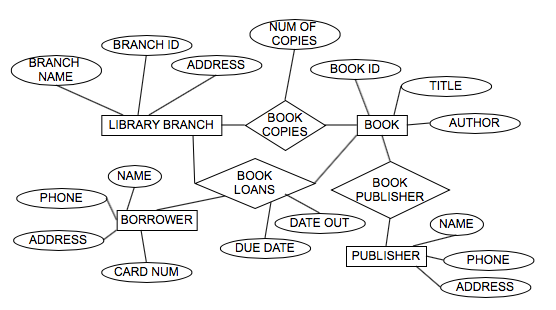
\includegraphics[width=15cm]{images/9-3.png}
\end{center}

Book authors, in this particular diagram, are represented as a multi-valued attribute of books.